
\part{Working with ImageJ\label{part:Working-with-ImageJ}}

This part introduces some basic aspects of ImageJ so that you can
use the software more efficiently. It also introduces some important
terms and concepts used throughout this guide. You may skip it if
you already use the program efficiently and are familiar with terms
such as \nameref{sub:Virtual-Stacks}, \nameref{sub:Hyperstacks-Intro},
\nameref{sub:Pseudocolor-Images}, \nameref{sub:Color-Composites}
or \nameref{sub:Composite-selections}.


\section{Using Keyboard Shortcuts\label{sub:Using-Shortcuts}}

You'll learn more and more \index{Keyboard@Keyboard \see{Shortcuts and Modifier keys,}}\index{Shortcuts}shortcut
keys as you use ImageJ, because (almost) all shortcuts are listed
throughout ImageJ menus. Similarly, in this guide each command has
its shortcut key listed on its name (flanked by square brackets).
Please note that the notation for these key-bindings is case sensitive,
i.e., Shift-modifiers are not explicitly mentioned (a capital \textsf{A}
means \textsf{Shift--A}) and assumes that \emph{Require control key
for shortcuts }in \textsf{\userinterface{\textsf{Edit\lyxarrow{}Options\lyxarrow{}\nameref{sub:Misc...}}}}
is unchecked (i.e., except when using the IJ \nameref{sub:ImageJ-Macro-Editor}
or the \nameref{sec:Text-Tool}, you won't have to hold down the Control
key to use menu shortcuts). For example, the command \textsf{\userinterface{\textsf{Edit\lyxarrow{}\nameref{sub:Invert-[I]}}}}
can be evoked by \mykeystroke{Shift} \mykeystroke{I} or \mykeystroke{Ctrl}
\mykeystroke{Shift} \mykeystroke{I} if \emph{Require control key
for shortcuts }is checked. The full list of ImageJ shortcuts (\emph{see}
\nameref{sec:Keyboard-Shortcuts}) can be retrieved at any time using
the \textsf{\userinterface{\textsf{Plugins\lyxarrow{}Utilities\lyxarrow{}\nameref{sub:List-Shortcuts...}}}}
command.

There are three \index{Modifier keys}modifier keys in ImageJ:
\begin{lyxlist}{00.00.0000}
\item [{\textbf{Control}}] (\textbf{Command Key}\index{Command key} on
Apple keyboards) Denoted by `Ctrl'\nomenclature{Ctrl}{Control key. In this guide also the Command key in Apple keyboards}
or \mykeystroke{Ctrl} in this document. Although a control key is
typically present on Apple keyboards, on a Macintosh computer running
ImageJ the Command key \mykeystroke{\cmd\  Cmd} replaces the functionality
of the Control key of other operating systems. For sake of simplification,
`Ctrl' will always refer to both  throughout this guide.
\item [{\textbf{Shift}}] Denoted by `Shift'\nomenclature{Shift}{Shift key}
or \mykeystroke{Shift} in this document.
\item [{\textbf{Alt}}] Denoted by `Alt'\nomenclature{Alt}{Alt, Option or Meta key}
or \mykeystroke{Alt} in this document. This is also the `Option'
or `Meta' key on many keyboards. In ImageJ, it is also used to type
special unit symbols such as $\micro$ (\mykeystroke{Alt}\mykeystroke{M})
or $\angstrom$ (\mykeystroke{Alt}\mykeystroke{Shift}\mykeystroke{A}). 
\end{lyxlist}

\calso{\nameref{sec:Keyboard-Shortcuts}, \userinterface{Plugins\lyxarrow{}\nameref{sub:Shortcuts}}}

\begin{infobox}
\caption{\label{infobox:Frontmost-window}Frontmost Window and Window Activation}


\noindent In ImageJ, all operations are performed on the active (frontmost)
image (which has its title bar highlighted). If a window is already
open it will activate when its opening command is re-run, e.g., if
the B\&C window is already opened (\userinterface{\noindent Image\lyxarrow{}Adjust\lyxarrow{}\nameref{sub:Brightness/Contrast...[C]}}),
pressing its keyboard shortcut (\,\mykeystroke{\noindent Shift}
\mykeystroke{C}\,) will activate it. \medskip{}


\noindent Pressing \mykeystroke{\noindent Enter} on any image will
bring the \nameref{fig:The-ImageJ-window} to the foreground. In addition,
it is also possible to permanently place the main window above all
other windows (\emph{see}  \nameref{sub:FloatingMainWin}).
\end{infobox}



\section{Finding Commands\label{sec:Finding-Commands}}

Navigating through the extensive list of ImageJ commands, macros and
plugins may be quite cumbersome. Through its built-in Command Finder\,/\,Launcher\cite{C-ComandFinder},
ImageJ offers an expedite alternative that allows you to retrieve
commands extremely fast: \textsf{\userinterface{\textsf{Plugins\lyxarrow{}Utilities\lyxarrow{}\nameref{sub:Command-Finder}}}}.

In addition, ImageJ features a find function that locates macros,
scripts and plugins source (\filenameref{.java}) files on your computer:
the \textsf{\userinterface{\textsf{Plugins\lyxarrow{}Utilities\lyxarrow{}\nameref{sub:Search...}}}}
command. Because most of IJ source files contain circumstanced comments,
you can use this utility to retrieve files related not only to a image
processing routine (e.g.,\emph{ background }or\emph{ co-localization})
but also to a practical context such as \emph{radiogram}, \emph{cell}
or \emph{histology}. Indeed, ImageJ source files contain detailed
annotations useful to both developers and regular users that want
to know more about ImageJ routines and algorithms.

\textsf{\userinterface{\textsf{\nameref{sub:Search...}}}} and \textsf{\userinterface{\textsf{\nameref{sub:Command-Finder}}}}
are described in detail in \textsf{\userinterface{\textsf{Plugins\lyxarrow{}\nameref{sub:Utilities}}}}.
\begin{figure}
\noindent \begin{centering}
\hspace{11.1em}\textsf{\small Plugins\lyxarrow{}Utilities\lyxarrow{}\nameref{sub:Command-Finder}\vspace{3pt}
}
\par\end{centering}{\small \par}

\noindent \begin{centering}
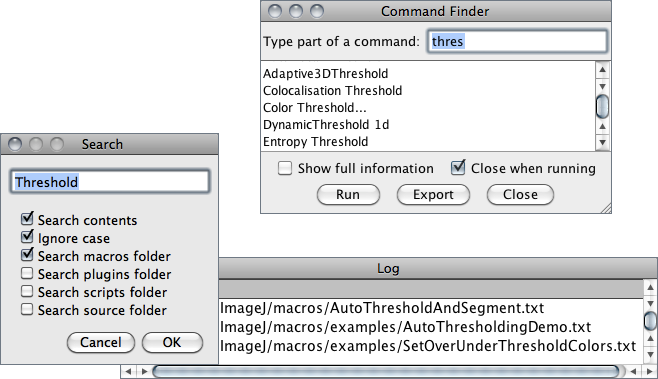
\includegraphics[scale=0.55]{images/CommandFinderAndSearch}
\par\end{centering}

\noindent \centering{}\textsf{\small Plugins\lyxarrow{}Utilities\lyxarrow{}\nameref{sub:Search...}}
\end{figure}



\calso{\nameref{sub:Control-Panel...}, \nameref{sec:Keyboard-Shortcuts}
and \filenameref{\href{http://imagej.nih.gov/ij/macros/SourceCodeRetriever.txt}{SourceCodeRetriever}},
a macro that searches for a menu entry and retrieves the source file
of the respective command}


\section[Undo and Redo]{Undo and Redo\label{sec:Undo-and-Redo}}

Probably the first thing you will notice is that ImageJ does not have
a large \index{Undo}undo/redo buffer. Undo (\textsf{\userinterface{\textsf{Edit\lyxarrow{}\nameref{sub:Undo-[z]}}}})
is currently limited to the most recent image editing\,/\,filtering
operation. With time you will appreciate that this is necessary to
minimize memory overhead. Nevertheless, with IJ\,1.45 and later,
\textsf{\userinterface{\textsf{\nameref{sub:Undo-[z]}}}} is, in most
cases, undoable and can be applied to multiple images if \emph{Keep
multiple undo buffers }is checked in \textsf{\userinterface{\textsf{Edit\lyxarrow{}Options\lyxarrow{}\nameref{sub:Memory-&-Threads...}}}}

If you cannot recover from a mistake, you can always use \textsf{\userinterface{\textsf{File\lyxarrow{}\nameref{sub:Revert[r]}}}}
to reset the image lo its last saved state. For selections, \textsf{\userinterface{\textsf{Edit\lyxarrow{}Selection\lyxarrow{}\nameref{sub:Restore-Selection-[E]}}}}
can be used to recover any misdealt selection.

In ImageJ the equivalent to \index{Redo}`Redo' is the \textsf{\userinterface{\textsf{Process\lyxarrow{}\nameref{sub:Repeat-Command-[R]}}}},
that re-runs the previous used command (skipping \textsf{\userinterface{\textsf{Edit\lyxarrow{}\nameref{sub:Undo-[z]}}}}
and \textsf{\userinterface{\textsf{File\lyxarrow{}\nameref{sub:Open...}}}}
commands).


\calso{\textsf{\userinterface{\textsf{Plugins\lyxarrow{}Utilities\lyxarrow{}\nameref{sub:Reset...}}}},
\href{http://imagejdocu.tudor.lu/doku.php?id=plugin:utilities:multi_undo:start}{Multi Undo}
plugin}


\section{Image Types and Formats\label{sec:Image-Types}}

\index{Image types}Digital Images are two-dimensional grids of pixel\nomenclature{pixel}{Picture element}
intensities values with the width and height of the image being defined
by the number of pixels in $x$ (rows) and $y$ (columns) direction.
Thus, pixels (picture elements) are the smallest single components
of images, holding numeric values -- pixel intensities -- that range
between black and white. The characteristics of this range, i.e.,
the number of unique intensity (brightness) values that can exist
in the image is defined as the bit\nomenclature{bit}{Binary digit}--depth
of the image and specifies the level of precision in which intensities
are coded, e.g.: A 2--bit image has $2^{2}=4$\,tones: 00 (black),
01 (gray), 10 (gray), and 11 (white). A 4--bit image has $2^{4}=16$\,tones
ranging from 0000 (0) to 1111 (16), etc. In terms of bits per pixel
(bpp\nomenclature{bpp}{Bits per pixel}), the most frequent types
of images (\userinterface{Image\lyxarrow{}\nameref{sub:Type}}) that
ImageJ deals with are (\index{ImageJ2}\nameref{sub:ImageJ2intro}
supports \href{http://imagejdev.org/imagej2-pixel-types}{many more types of image data}):
\begin{lyxlist}{RGB-Color---}
\item [{\textbf{8--bit}}] \noindent Images that can display 256 ($2^{8}$)
gray levels (integers only).
\item [{\textbf{16--bit}}] \noindent Images that can display 65,\,536
($2^{16}$) gray levels (integers only).
\item [{\textbf{32--bit}}] \noindent Images that can display 4,\,294,\,967,\,296
($2^{32}$) gray levels (integers and fractional values). 32--bit
images pixels can have\textsc{ any} intensity value (i.e., any real
number) including \emph{NaN}\nomenclature{NaN}{Not a Number} (Not
a Number). In computing these are called floating point images.
\item [{\textbf{RGB\ Color}}] \noindent \nameref{sec:Color-Images} that
can display 256 values in the \uline{R}ed, \uline{G}reen and
\uline{B}lue channel. These are 24--bit ($2^{3\times8}$) images.
RGB\nomenclature{RGB}{Red Green Blue} color images can also be 32--bit
color images (24--bit color images with additional eight bits coding
alpha blending values, i.e., transparency).
\end{lyxlist}

\subsection*{Native Formats\label{sub:Native-Formats}}

Natively (i.e.\ without the need of third-party plugins) ImageJ opens
the following formats: \textbf{TIFF}\nomenclature{TIFF}{Tagged Image File Format},
\textbf{GIF}\nomenclature{GIF}{Graphics Interchange Format}, \textbf{JPEG}\nomenclature{JPEG}{Joint Photographic Experts Group},
\textbf{PNG}\nomenclature{PNG}{Portable Network Graphics}, \textbf{DICOM}\nomenclature{DICOM}{Digital Imaging and Communications in Medicine},
\textbf{BMP}\nomenclature{BMP}{Bitmap Image File (Device Independent Bitmap, DIB)},
\textbf{PGM}\nomenclature{PGM}{Portable GrayMap} and \textbf{FITS}\nomenclature{FITS}{Flexible Image Transport System}.
\index{Image formats!Native}Many more formats are supported with
the aid of plugins. These are discussed in \nameref{sub:Non-native-Supported-Formats}.
\begin{lyxlist}{00.00.0000}
\item [{\textbf{TIFF}}] (Tagged Image File Format) is the `default' format
of ImageJ (cf.\ \textsf{\userinterface{\textsf{File\lyxarrow{}\nameref{sub:Save[s]}}}}).
Images can be 1--bit, 8--bit, 16--bit (unsigned%
\footnote{A numeric variable is signed if it can represent both positive and
negative numbers, and unsigned if it can only represent positive numbers.%
}), 32--bit (real) or RGB color. \index{TIFF}TIFF files with multiple
images of the same type and size open as \nameref{sub:Stacks-Intro}
or \nameref{sub:Hyperstacks-Intro}. ImageJ opens \index{Lossless compression}lossless
compressed TIFF files (\emph{see} \ref{infobox:Formats} \nameref{infobox:Formats})
by the LZW\nomenclature{LZW}{Lempel-Ziv-Welch}\index{LZW compression},
\index{PackBits compression}PackBits and \index{ZIP!Lossless compression}ZIP
(\index{Deflate@Deflate \see{Zip compression,}}Deflate/Inflate) \cite{C-ZIPcompressedTIFFs}
compression schemes. In addition, TIFF files can be opened and saved
as \index{ZIP!Archived TIFF files}ZIP archives.\\
Tiff tags and information needed to import the file (number of images,
offset to first images, gap between images) are printed to the \nameref{sec:Log-Window}
when ImageJ is running in \emph{Debug Mode} (\userinterface{Edit\lyxarrow{}Options\lyxarrow{}\nameref{sub:Misc...}},
\emph{see} \nameref{sec:Settings-and-Preferences}).
\item [{\textbf{DICOM}}] (Digital Imaging and Communications in Medicine)
is a standard popular in the medical imaging community. Support in
ImageJ is limited to uncompressed \index{DICOM}DICOM files. DICOM
files containing multiple images open as \nameref{sub:Stacks-Intro}.\\
Use \textsf{\userinterface{\textsf{Image\lyxarrow{}\nameref{sub:Show-Info...}}}}
to display the DICOM header information. A DICOM sequence can be opened
using \textsf{\userinterface{\textsf{File\lyxarrow{}Import\lyxarrow{}\nameref{sub:Image-Sequence...}}}}
or by dragging and dropping the folder on the `ImageJ' window. Imported
sequences are sorted by image number instead of filename and the tags
are preserved when DICOM images are saved in TIFF format. ImageJ supports
custom DICOM dictionaries, such as the one at \url{http://imagej.nih.gov/ij/download/docs/DICOM_Dictionary.txt}.
More information can be found at the \href{http://www.cabiatl.com/mricro/dicom/index.html}{Center for Advanced Brain Imaging}.
\item [{\textbf{FITS}}] (Flexible Image Transport System) image is the
format adopted by the astronomical community for data interchange
and archival storage. Use \textsf{\userinterface{\textsf{Image\lyxarrow{}\nameref{sub:Show-Info...}}}}
to display the \index{FITS}FITS header. More information \href{http://fits.gsfc.nasa.gov}{here}.
\item [{\textbf{PGM}}] (\index{PGM}Portable GrayMap), \textbf{PBM\nomenclature{PBM}{Portable BitMap}}
(Portable BitMap) and \textbf{PPM\nomenclature{PPM}{Portable PixMap}}
(Portable PixMap) are simple image formats that use an ASCII\nomenclature{ASCII}{American Standard Code for Information Interchange}
header. More information \href{http://local.wasp.uwa.edu.au/~pbourke/dataformats/ppm/}{here}.
\item [{\textbf{AVI}}] (Audio Video Interleave) is a container format which
can contain data encoded in many different ways. ImageJ only supports
uncompressed \index{AVI}AVIs, various \index{YUV}YUV 4:2:2 compressed
formats, and \index{PNG}PNG or \index{JPEG}JPEG-encoded individual
frames. Note that most \index{MJPG}MJPG\nomenclature{MJPG}{Motion-JPEG}
(motion-JPEG) formats are not read correctly. Attempts to open AVIs
in other formats will fail.
\end{lyxlist}

\calso{\nameref{sub:Non-native-Supported-Formats}, \ref{infobox:Formats}
\nameref{infobox:Formats}, \ref{infobox:JpegAlert} \nameref{infobox:JpegAlert}}


\subsection*{Non--native Formats \label{sub:Non-native-Supported-Formats}}

When opening a file, ImageJ first checks whether it can natively handle
the format. \index{Image formats!Non--native}If ImageJ does not recognize
the type of file it calls for the appropriate reader plugin using
\href{http://imagej.nih.gov/ij/plugins/file-handler.html}{HandleExtraFileTypes},
a plugin bundled with ImageJ. If that fails, it tries to open the
file using the \index{LOCI Bio-Formats}\index{Bio-formats@Bio-formats \see{LOCI,}}\href{http://www.loci.wisc.edu/ome/formats.html}{LOCI Bio-Formats library}
(if present), a remarkable plugin that supports around \href{http://www.loci.wisc.edu/software/bio-formats}{eighty of the most common}
file formats used in microscopy. If nevertheless the file cannot be
opened, an error message is displayed. Because both these plugins
are under active development, it is important that you keep them updated.

In addition, the ImageJ web site lists \href{http://imagej.nih.gov/ij/plugins/\#io}{more than fifty plugins}
that recognize more `exotic' file formats. The ImageJ Documentation
Portal maintains a \href{http://imagejdocu.tudor.lu/doku.php?id=faq:general:which_file_formats_are_supported_by_imagej}{list of file formats}
that are supported by ImageJ.


\calso{\nameref{sub:Native-Formats}, \textsf{\userinterface{\textsf{File\lyxarrow{}\nameref{sub:Import}}}},
\ref{infobox:Formats} \nameref{infobox:Formats}, \ref{infobox:JpegAlert}
\nameref{infobox:JpegAlert}, \href{http://imagej.nih.gov/ij/plugins/\#acq}{Acquisition plugins},
\href{http://imagej.nih.gov/ij/plugins/\#io}{Input/Output plugins}}

\begin{infobox}
\caption{\label{infobox:Formats}Image Types: Lossy Compression and Metadata}


\noindent Two critical aspects to keep in mind when converting images:
\begin{description}
\item [{\label{misc:LossyCompression}Lossy\ compression}] Transcoding
an image into a format that uses \index{Lossy compression}lossy compression
will alter the original data, introducing artifacts (\emph{see} \ref{infobox:JpegAlert}
\nameref{infobox:JpegAlert}). This is the case, e.g., for JPEG formats
(with the exception of some \index{JPEG2000@{\small JPEG2000}}JPEG2000
images that use lossless compression). As such, these types of data
are intended for human interpretation only and are not suitable for
quantitative analyses
\item [{\label{misc:Metadata}Metadata}] In ImageJ, \index{Metadata}metadata
associated with the image, such as scale, gray value calibration and
user comments is only supported in tiff and zip (compressed tiff)
images. In addition, selections and \nameref{sub:Overlay-Intro} are
also saved in the TIFF header (cf.\ \textsf{\userinterface{File\lyxarrow{}\nameref{sub:Save[s]}}}).
None of the above is saved in other formats (cf.\ \nameref{sub:Native-Formats}).\end{description}
\end{infobox}



\section{Stacks, Virtual Stacks and Hyperstacks\label{sec:StacksVirtualStacksHyperStks}}


\subsection*{Stacks\label{sub:Stacks-Intro}}

ImageJ can display multiple spatially or temporally related images
in a single window. These image sets are called stacks. The images
that make up a stack are called slices. In \index{Stacks}stacks,
a pixel (which represents 2D image data in a bitmap image) becomes
a voxel\nomenclature{voxel}{Volumetric pixel} (volumetric pixel),
i.e., an intensity value on a regular grid in a three dimensional
space. 

All the slices in a stack must be the same size and bit depth. A scrollbar
provides the ability to move through the slices and the slider is
preceded by a play/pause icon that can be used to start/stop stack
animation. Right-clicking on this icon runs the \userinterface{\nameref{sub:Animation-Options...}}
dialog box.

Most ImageJ filters will, as an option, process all the slices in
a stack. ImageJ opens multi-image TIFF files as a stack, and saves
stacks as multi-image TIFFs. The \userinterface{\textsf{File\lyxarrow{}Import\lyxarrow{}}\nameref{sub:Import>Raw}}
command opens other multi-image, uncompressed files. A folder of images
can be opened as a stack either by dragging and dropping the folder
onto the `ImageJ' window or or by choosing \userinterface{\textsf{File\lyxarrow{}Import\lyxarrow{}}\nameref{sub:Image-Sequence...}}
To create a new stack, simply choose \userinterface{File\lyxarrow{}New\lyxarrow{}\nameref{sub:Image...[n]}}
and set the \emph{Slices} field to a value greater than one. The \userinterface{Image\lyxarrow{}\nameref{sub:Stacks}}
submenu contains commands for common stack operations.
\begin{figure}
\noindent \includegraphics[scale=0.55]{images/StacksHyperstacks}\caption[Stacks and Hyperstacks]{\label{fig:Stacks-and-Hyperstacks}\textbf{Stacks and Hyperstacks
in ImageJ:}\textsf{ }\protect\userinterface{File\lyxarrow{}Open Samples\lyxarrow{}Mitosis (26MB, 5D stack)}.
Hyperstacks dimensionality can be reduced using the \protect\userinterface{Image\lyxarrow{}Hyperstacks\lyxarrow{}\nameref{sub:Reduce-Dimensionality...}},
\protect\userinterface{Image\lyxarrow{}Stacks\lyxarrow{}\nameref{sub:Z-Project...}}
or \protect\userinterface{Image\lyxarrow{}Hyperstacks\lyxarrow{}\nameref{sub:Channels...[Z]}}
commands. The `(V)' on the window titles denotes a virtual image
(\emph{see} \nameref{sub:Virtual-Stacks}).}
\end{figure}



\calso{\nameref{sub:StacksMenu}, \href{ http://fiji.sc/wiki/index.php/Stack_Manipulation}{Stack Manipulations}
on Fiji website, \href{http://imagej.nih.gov/ij/plugins/image5d.html}{Image5D}}


\subsection*{Virtual Stacks\label{sub:Virtual-Stacks}}

\index{Stacks!Virtual}\index{Virtual stacks@Virtual stacks \see{Stacks~(Virtual),}}Virtual
stacks are disk resident (as opposed to RAM\nomenclature{RAM}{Random-Access Memory}
resident) and are the only way to load image sequences that do not
fit in RAM. There are several things to keep in mind when working
with virtual stacks:
\begin{itemize}
\item Virtual stacks are read-only, so changes made to the pixel data are
not saved when you switch to a different slice. You can work around
this by using macros (e.g., {\small \href{http://imagej.nih.gov/ij/macros/Process_Virtual_Stack.txt}{Process Virtual Stack}})
or the \textsf{\userinterface{\textsf{Process\lyxarrow{}Batch\lyxarrow{}\nameref{sub:Virtual-Stack...}}}}
command
\item You can easily run out of memory using commands like \textsf{\userinterface{\textsf{Image\lyxarrow{}}\nameref{sub:Crop-[X]}}}
because any stack generated from commands that do not generate virtual
stacks will be RAM resident.
\item TIFF virtual stacks can usually be accessed faster than \index{JPEG}JPEG
virtual stacks. A JPEG sequence can be converted to TIFF by opening
the JPEG images as a virtual stack and using \textsf{\userinterface{\textsf{File\lyxarrow{}Save As\lyxarrow{}}\nameref{sub:SaveAs>Image-Seq...}}}
to save in TIFF format
\end{itemize}
ImageJ appends a `(V)' to the window title of virtual stacks and
hyperstacks (\emph{see} \nameref{sub:Hyperstacks-Intro}). Several
built-in ImageJ commands in the \textsf{\userinterface{\textsf{File\lyxarrow{}}\nameref{sub:Import}}}
submenu have the ability to open virtual stacks, namely: \userinterface{\nameref{sub:Import>TIFF-Virtual-Stack}},
\userinterface{\nameref{sub:Image-Sequence...}}, \userinterface{\nameref{sub:Import>Raw}},\textsf{
}\userinterface{\nameref{sub:Stack-From-List...}},\textsf{ }\userinterface{\nameref{sub:Import>AVI...}}
(cf.\ \href{http://imagej.nih.gov/ij/plugins/virtual-opener.html}{Virtual Stack Opener}).
In addition, TIFF stacks can be open as virtual stacks by drag and
drop (cf.\ \ref{infobox:VirtualTiff} \nameref{infobox:VirtualTiff}).


\calso{\href{http://www.loci.wisc.edu/ome/formats.html}{LOCI Bio-Formats}
and \href{http://fiji.sc/wiki/index.php/Register_Virtual_Stack_Slices}{RegisterVirtualStackSlices}
plugins, \href{http://imagej.nih.gov/ij/macros/Process_Virtual_Stack.txt}{Process Virtual Stack}
and \href{http://imagej.nih.gov/ij/macros/VirtualStackFromList.txt}{VirtualStackFromList}
macros }

\begin{infobox}
\caption{\label{infobox:VirtualTiff}Opening Virtual Stacks by Drag \& Drop}


\noindent TIFF stacks with a \filenameref{\noindent .tif} extension
open as virtual stacks when dragged and dropped on the\textsf{~
\includegraphics[scale=0.5]{images/tools/Switcher-small}~}toolbar
icon.\medskip{}


\noindent \centering{}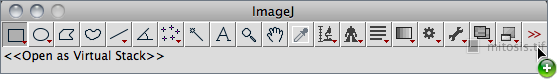
\includegraphics[scale=0.55]{images/DragAndDropVirtualTiff}
\end{infobox}



\subsection*{Hyperstacks\label{sub:Hyperstacks-Intro}}

\index{Stacks!Hyperstacks}Hyperstacks are multidimensional images,
extending image stacks to four (4D) or five (5D) dimensions: $x$
(width), $y$ (height), $z$ (slices), $c$ (channels or wavelengths)
and $t$ (time frames). Hyperstacks are displayed in a window with
three labelled scrollbars (\emph{see} \nameref{fig:Stacks-and-Hyperstacks}).
Similarly to the scrollbar in \nameref{sub:Stacks-Intro}, the frame
slider (\emph{t}) has a play/pause icon. 


\calso{\userinterface{\textsf{Image}\lyxarrow{}\nameref{sub:Hyperstacks}}
submenu}


\section[Color Images]{Color Images%
\footnote{This section is partially extracted from the MBF\,ImageJ online manual
at \protect\url{http://www.macbiophotonics.ca/imagej/colour_image_processi.htm}.%
}\label{sec:Color-Images}}

\index{MBF ImageJ}ImageJ deals with color mainly in three ways: pseudocolor
images, RGB images, RGB/ HS{\small B\nomenclature{HSB}{Hue Saturation Brightness}}
stacks, and composite images.\index{Image types}


\subsection*{Pseudocolor Images\label{sub:Pseudocolor-Images}}

A pseudocolor (or indexed color) image is a single channel gray image
(8, 16 or 32--bit) that has color assigned to it via a lookup table
or LUT\nomenclature{LUT}{Lookup table}\index{LUT}. A LUT is literally
a predefined table of gray values with matching red, green and blue
values so that shadows of gray are displayed as colorized pixels.
Thus, differences in color in the pseudo-colored image reflect differences
in intensity of the object rather than differences in color of the
specimen that has been imaged.

8-bit indexed color images (such as GIFs) are a special case of pseudocolor
images as their lookup table is stored in the file with the image.
These images are limited to 256 colors (24--bit RGB images allow 16.7
million of colors, \emph{see} \nameref{sec:Image-Types}) and concomitantly
smaller file sizes. Reduction of true color values to a 256 \index{Color palette@Color palette \see{LUT,}}color
palette is performed by color quantization algorithms. ImageJ uses
the \index{Color!Quantization}\index{Heckbert quantization}\index{Algorithm!Heckbert quantization}Heckbert's
median-cut color quantization algorithm (\emph{see} \userinterface{Image\lyxarrow{}\nameref{sub:Type}}
menu), which, in most cases, allows indexed color images to look nearly
identical to their 24-bit originals.


\calso{\userinterface{\textsf{Image}\lyxarrow{}\nameref{sub:Lookup-Tables}}
and \nameref{sub:LUTMenu}}


\subsection*{True Color Images\label{sub:True-color-images}}

As described in \nameref{sec:Image-Types}, true color images such
as RGB images reflect genuine colors, i.e., the green in an RGB image
reflects green color in the specimen. Color images are typically produced
by color CCD\nomenclature{CCD}{Charge-Coupled Device} cameras, in
which \index{Color filter array}color filter arrays (\href{http://en.wikipedia.org/wiki/Bayer_filter}{Bayer masks})
are placed over the image sensor.\index{CCD}


\subsubsection*{Color Spaces and Color Separation\label{sub:Color-Spaces-and}}

\href{http://en.wikipedia.org/wiki/Color_space}{Color spaces} \index{Color!Models}describe
the gamut of colors that image-handling devices deal with. Because
human vision is trichromatic, most color models represent colors by
three values. Mathematically, these values (color components) form
a three-dimensional space such as the RGB\index{RGB}, \index{HSB}HSB,
\index{CIE Lab}CIE\,Lab or \index{YUV}YUV color space. 
\begin{figure}[H]
\noindent 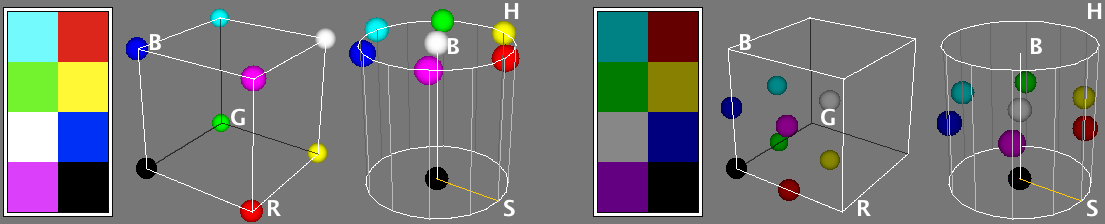
\includegraphics[width=1\columnwidth]{images/RGB-HSBcolorModels}\caption[RGB and HSB color models]{\textbf{\label{fig:ColorModels}Representation of an eight pixel
color image in the RGB and HSB color spaces.} The RGB color space
maps the RGB color model to a cube with \emph{Red} (R) values increasing
along the x-axis, \emph{Green} (G) along the y-axis and \emph{Blue}
(B) along the z-axis. In the HSB cylindrical coordinate system, the
angle around the central vertical axis corresponds to \emph{Hue} (H),
the distance from the axis corresponds to \emph{Saturation} (S), and
the distance along the axis corresponds to \emph{Brightness} (B).
In both cases the origin holds the black color. The right panel shows
the same image after brightness reduction, easily noted by the vertical
displacement along the HSB cylinder. Images produced using Kai Uwe
Barthel's \protect\href{http://www.f4.fhtw-berlin.de/~barthel/ImageJ/ColorInspector//help.htm}{3D Color Inspector}
plugin.}
\end{figure}


RGB (\uline{R}ed, \uline{G}reen, \uline{B}lue) is the most
commonly-used color space. However, other alternatives such as HSB
(\uline{H}ue, \uline{S}aturation, \uline{B}rightness) provide
significant advantages when processing color information. In the HSB
color space, \emph{Hue} describes the attribute of pure color, and
therefore distinguishes between colors. \emph{Saturation} (sometimes
called ``purity'' or ``vibrancy'') characterizes the shade of
color, i.e., how much white is added to the pure color.\emph{ Brightness}
(also know as \emph{Value} -- HSV system) describes the overall brightness
of the color (\emph{see} e.g., the color palette of \nameref{fig:CPtool}).
In terms of digital imaging processing, using the HSB system over
the traditional RGB is often advantageous: e.g., since the Brightness
component of an HSB image corresponds to the grayscale version of
that image, processing only the brightness channel in routines that
require grayscale images is a significant computational gain%
\footnote{\emph{See} Wootton R, Springall DR, Polak JM. Image Analysis in Histology:
Conventional and Confocal Microscopy. \emph{Cambridge University Press},
1995\emph{,} ISBN 0521434823%
}. You can read more about the HSB color model \href{http://en.wikipedia.org/wiki/HSB_color_space}{here}.

In ImageJ, conversions between image types are performed using the
\userinterface{\textsf{\small Image}\lyxarrow{}\nameref{sub:Type}}
submenu. Segmentation on the HSB, RGB, CIE\,Lab and YUV color spaces
can be performed by the \userinterface{\textsf{\small Image}\lyxarrow{}Adjust\lyxarrow{}\nameref{sub:Color-Threshold...}}
command \cite{C-ColorThres}. Segregation of color components (specially
useful for quantification of \index{Color!Deconvolution}\index{Color!Separation@Separation \see{Color!Deconvolution,}}\index{Immunohistochemistry@Immunohistochemistry \see{Histochemical staining,}}histochemical
staining) is also possible using Gabriel Landini's \href{http://www.dentistry.bham.ac.uk/landinig/software/cdeconv/cdeconv.html}{Colour Deconvolution}
plugin. In addition, several other plugins related to color processing
can be obtained from the \href{http://imagej.nih.gov/ij/plugins/index.html\#color}{ImageJ website}.


\subsubsection*{Conveying Color Information\textmd{}%
\footnote{This section is partially extracted from Masataka Okabe and Kei Ito,
\emph{Color Universal Design (CUD) --- How to make figures and presentations
that are friendly to Colorblind people}, \protect\url{http://jfly.iam.u-tokyo.ac.jp/color/},
accessed 2009.01.15%
}\label{sub:Conveying-Color-Information}}

People see color with significant variations. Indeed, the popular
phrase ``One picture is worth ten thousand words'' may not apply
to certain color images, specially those that do not follow the basic
principles of \href{http://jfly.iam.u-tokyo.ac.jp/color/}{Color Universal Design}.
Citing Masataka Okabe and Kei Ito:
\begin{quotation}
\index{Color!Blindness}Colorblind people can recognize a wide ranges
of colors. But certain ranges of colors are hard to distinguish. The
frequency of colorblindness is fairly high. One in 12 Caucasian (8\%),
one in 20 Asian (5\%), and one in 25 African (4\%) males are so-called
`red--green' colorblind.

There are always colorblind people among the audience and readers.
There should be more than \textsc{ten} colorblind in a room with 250\,people
(assuming 50\% male and 50\% {\small female}).

{[}\,\ldots{}{]} There is a good chance that the paper you submit
may go to colorblind reviewers. Supposing that your paper will be
reviewed by three white males (which is not unlikely considering the
current population in science), the probability that at least one
of them is colorblind is whopping 22\%! 
\end{quotation}
\begin{figure}
\noindent 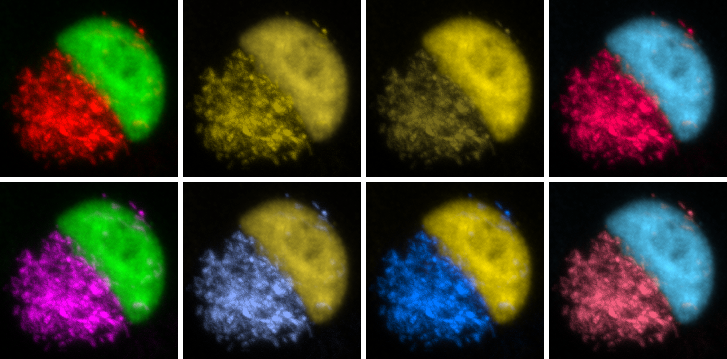
\includegraphics[width=1\columnwidth]{images/Dichromacy}\caption[Red--green images and partial color blindness]{\textbf{\label{fig:ColorBlindness}Red--green images and partial
color blindness.} Deuteranopia (second panel), protanopia (third panel)
are the most common types of partial color blindness (red\,/\,green
confusion). Tritanopia (blue\,/\,orange confusion, fourth panel)
is quite rare. \nameref{infobox:Replacing-Red-w-Magenta} (bottom
row) is a simple way to compensate for color vision deficiencies.}
\end{figure}
One practical point defined by the \href{http://jfly.iam.u-tokyo.ac.jp/color/}{Color Universal Design}
is the use of magenta in red--green overlays (\emph{see also} \cite{Landini:2009p19625}).
Magenta is the equal mixture of red and blue. Colorblind people that
have difficulties recognizing the red component can easily recognize
the blue hue. The region of double positive becomes white, which is
easily distinguishable for colorblind. In ImageJ this is easily accomplished
using the \userinterface{Image\lyxarrow{}Color\lyxarrow{}\nameref{sub:Merge-Channels...}},
or using the ImageJ macro language (\emph{see} \ref{infobox:Replacing-Red-w-Magenta}
\nameref{infobox:Replacing-Red-w-Magenta}). 
\begin{infobox}
\caption{\label{infobox:Replacing-Red-w-Magenta}Replacing Red with Magenta
in RGB Images}


When building RGB images, magenta can be obtained using the \userinterface{Image\lyxarrow{}Color\lyxarrow{}\nameref{sub:Merge-Channels...}}
Previously created RGB images can be converted to \index{Magenta Green Blue (MGB)}`MGB'
using \userinterface{Image\lyxarrow{}Color\lyxarrow{}\nameref{sub:Channels...[Z]}}.
Alternatively, the \textsf{\userinterface{\textsf{Process\lyxarrow{}\nameref{sub:Image-Calculator...}}}}
command can be used to add the red channel to the blue channel. Both
these approaches can be automated using the ImageJ macro language
as exemplified by Macros \eqref{lis:RGBtoMGB1} and \eqref{lis:RGBtoMGB2}.
Once saved in the \dirnameref{ImageJ/plugins/} folder these \nameref{sub:Macros-ExtendingIJ}
are treated as regular ImageJ commands.\medskip{}


In \nameref{sub:Fiji-intro}, as expected, the procedure of modifying
RGB images is simpler: one just needs to run \textsf{\userinterface{\textsf{Image\lyxarrow{}Color\lyxarrow{}Replace Red with Magenta}}}.
For even more convenience, Fiji provides an analogous command that
replaces the system clipboard's image with a magenta-green one.
\end{infobox}


It is also possible to simulate color blindness using the \href{http://www.vischeck.com/downloads/}{Vischeck}
or \href{http://www.dentistry.bham.ac.uk/landinig/software/dichromacy/dichromacy.html}{Dichromacy}
plugins%
\footnote{One advantage of Dichromacy over the Vischeck plugin is that it can
be recorded and called from scripts and macros, without user interaction.%
}, or in \index{Fiji}\nameref{sub:Fiji-intro}, using the \userinterface{Image\lyxarrow{}Color\lyxarrow{}Simulate Color Blindness}
command.
\begin{lstlisting}[caption={Replace\,Red\,with\,Magenta.ijm (Using \protect\userinterface{Process\lyxarrow{}Image Calculator\ldots{}})},label={lis:RGBtoMGB2},float=h,showstringspaces=false,tabsize=4]
 /* This macro replaces Red with Magenta in RGB images using Process>Image Calculator...  command. */
   if (bitDepth!=24)
       exit("This macro requires an RGB image");
 setBatchMode(true);
   title= getTitle();
   r= title+" (red)"; g= title+" (green)"; b= title+" (blue)";
   run("Split Channels");
   imageCalculator("Add", b, r);
   run("Merge Channels...", "red=&r green=&g blue=&b");
   rename(title + " (MGB)");
 setBatchMode(false);
\end{lstlisting}



\subsection*{Color Composite Images\label{sub:Color-Composites}}

In a \index{Color!Composites}composite image colors are handled through
channels. The advantages with this type of image over plain RGB images
are: 
\begin{enumerate}
\item Each channel is kept separate from the others and can be turned on
and off using the `Channels' tool (\textsf{\userinterface{\textsf{Image\lyxarrow{}Color\lyxarrow{}\nameref{sub:Channels...[Z]}}}}).
This feature allows, e.g., to perform measurements on a specific channel
while visualizing multiple. 
\item Channels can be 8, 16 or 32--bit and can be displayed with any lookup
table
\item More than 3\,channels can be merged or kept separate
\end{enumerate}
\begin{lstlisting}[caption={Replace\,Red\,with\,Magenta.ijm (Using \protect\userinterface{Image\lyxarrow{}Color\lyxarrow{}Channels\ldots{}})},label={lis:RGBtoMGB1},float=h,showstringspaces=false,tabsize=4]
 /* This macro replaces Red with Magenta in RGB images using the Image>Color>Channels... tool. */
   if (bitDepth!=24)         // Ignore non-RGB images
       exit("This macro requires an RGB image");
 setBatchMode(true);         // Enter `Batch' mode
   title = getTitle();       // Retrieve the image title
   run("Make Composite");    // Run Image>Color>Make Composite
   run("Magenta");           // Run Image>Lookup Tables>Magenta on channel 1
   run("RGB Color");         // Run Image>Type>RGB Color
   rename(title + " (MGB)"); // Rename the image
 setBatchMode(false);        // Restore `GUI' mode
\end{lstlisting}



\section{Selections\label{sec:Selections-Intro}}

Selections (regions of interest, ROIs\nomenclature{ROI}{Region Of Interest}),
are typically created using the \nameref{sub:Toolbar} \nameref{sec:IJ-Tools}.
Although ImageJ can display simultaneously several \index{Selection}\index{ROI@ROI \see{Selection,}}ROIs
(see \nameref{sub:Overlay-Intro} and \nameref{fig:The-ROI-Manager})
only one selection can be active at a time. Selections can be measured
(\textsf{\userinterface{\textsf{Analyze\lyxarrow{}}\nameref{sub:Measure...[m]}}}),
drawn (\userinterface{\textsf{Edit\lyxarrow{}}\nameref{sub:Draw-[d]}}),
filled (\textsf{\userinterface{\textsf{Edit\lyxarrow{}}\nameref{sub:Fill-[f]}}})
or filtered (\userinterface{\textsf{Process\lyxarrow{}}\nameref{sub:Filters}}
submenu), in the case of area selections. In addition it is also possible
to hold multiple ROIs as non-destructive \nameref{sub:Overlay-Intro}.

Selections can be initially outlined in one of the nine ImageJ default
colors (\emph{Red}, \emph{Green}, \emph{Blue}, \emph{Magenta}, \emph{Cyan},
\emph{Yellow}, \emph{Orange}, \emph{Black} and White). Once created,
selections can be contoured or painted with any other color using\textsf{
\userinterface{\textsf{Edit\lyxarrow{}Selection\lyxarrow{}}\nameref{sub:Properties...}}}.
Selection Color can be changed in \userinterface{\textsf{Edit\lyxarrow{}Options\lyxarrow{}}\nameref{sub:Colors...}},
by double clicking on the \nameref{sec:Point-Tool}, or using hot
keys (\emph{see} \eqref{lis:ChangeSelectionColor} \nameref{lis:ChangeSelectionColor}).
It is highlighted in the center of the \nameref{sec:Point-Tool} and
\nameref{sec:Multi-point-Tool}.
\begin{figure}[h]
\noindent 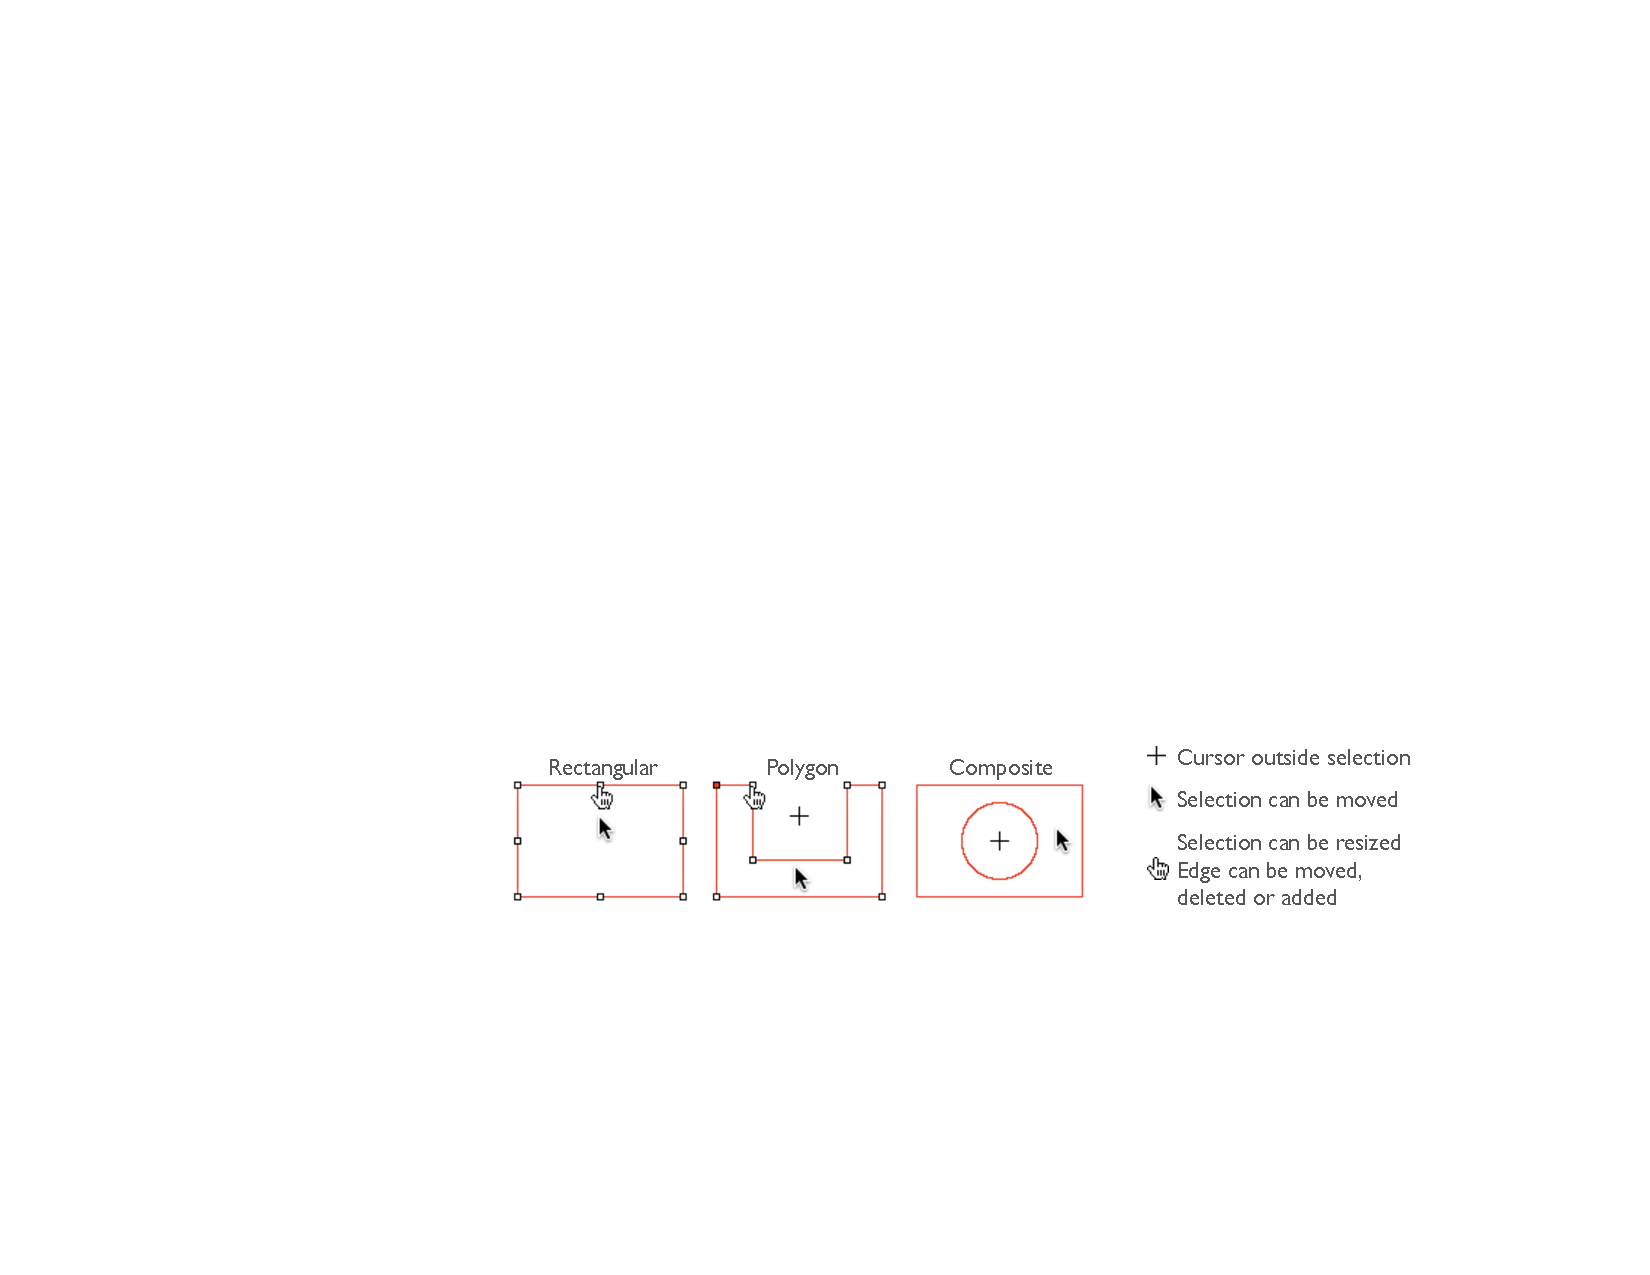
\includegraphics[width=0.88\columnwidth]{images/Selections}\caption{\textbf{\label{fig:exampleAreaROIs}Three types of area selections
In ImageJ.} Notice the cursor changes: to an \emph{arrow} when it
is within the selection, to a \emph{cross-hair} when outside the selection,
to a \emph{hand} when over a selection vertex or `handler'. Notice
also the filled handler in the polygon selection and the absence of
point handlers in \nameref{sub:Composite-selections}. \nameref{sub:Overlay-Intro},
i.e., non-active selections displayed in the non-destructive image
overlay, are also displayed without handlers.}
\end{figure}



\subsection{Manipulating ROIs\label{sub:Manipulating-ROIs}}

Most of commands that can be useful in defining or drawing selections
are available in the \textsf{\userinterface{\textsf{Edit\lyxarrow{}}\nameref{sub:SelectionSubMenu}}}
submenu and summarized in \nameref{fig:ROI-manipulations}. Listed
below are the most frequent manipulations involving \index{ROI@ROI \seealso{Selection,}}selections:
\begin{lyxlist}{00000000000}
\item [{\textbf{Adjusting}}] \noindent Area selections can be adjusted
with the \nameref{sub:Brush-Selection-Tool}. In addition, vertexes
of selections created with the \nameref{sub:Polygon-Selection-Tool}
and \nameref{sub:Segmented-Line-Selection} can be adjusted by Alt/Shift-clicking.
\item [{\textbf{Deleting}}] \noindent Choose any of the selection tools
and click outside the selection, or use \textsf{\userinterface{\noindent \textsf{Edit\lyxarrow{}Selection\lyxarrow{}}\nameref{sub:Select-None-[A]}}}.
Use\textsf{ \userinterface{\noindent \textsf{Edit\lyxarrow{}Selection\lyxarrow{}}\nameref{sub:Restore-Selection-[E]}}}
to restore a selection back after having deleted it. With \nameref{sub:Overlay-Intro},
an activated ROI can be deleted by pressing the \mykeystroke{\noindent Backspace}
(\mykeystroke{\noindent Delete} on Mac) key.
\item [{\textbf{Managing}}] \noindent A selection can be transferred from
one image window to another by activating the destination window and
runnig \textsf{\userinterface{\noindent \textsf{Edit\lyxarrow{}Selection\lyxarrow{}}\nameref{sub:Restore-Selection-[E]}}}.
Alternatively, \textsf{\userinterface{\noindent \textsf{Analyze\lyxarrow{}Tools\lyxarrow{}}\nameref{sub:SynchronizeWindows}}}
to create ROIs across multiple images. Multiple selections can be
stored as \nameref{sub:Overlay-Intro} or in the \nameref{fig:The-ROI-Manager}
list (\textsf{\userinterface{\noindent \textsf{Analyze\lyxarrow{}Tools\lyxarrow{}}\nameref{sub:ROI-Manager...}}}).
\item [{\textbf{Moving}}] \noindent Selections can be moved by clicking
and dragging as long as the cursor is within the selection and has
changed to an\ 
\includegraphics[scale=0.5]{images/pointers/Pointer-Arrow}.
The status bar displays the coordinates of the upper left corner of
the selection (or the bounding rectangle for non-rectangular selections)
as it is being moved. To move the contents of a selection, rather
than the selection itself, \textsf{\userinterface{\noindent \textsf{Edit\lyxarrow{}\nameref{sub:Copy[c]}}}},
\textsf{\userinterface{\noindent \textsf{Edit\lyxarrow{}\nameref{sub:Paste[v]}}}},
and then click within the selection and drag.
\item [{\textbf{Nudging}}] \noindent Selections can be `nudged' one pixel
at a time in any direction using the arrow keys. Note that the up
and down keys zoom the image in and out in the absence of selections
(\emph{see} \nameref{Arrow-Keys} shortcuts).
\item [{\textbf{Resizing}}] The \nameref{sub:Brush-Selection-Tool} can
be used to perform fine adjustments of ROI contours. Most ROIs can
be resized one pixel at a time by holding \mykeystroke{Alt} while
using the arrow keys. In general (\emph{see} \nameref{sec:Area-selection-tools}
and \nameref{sec:Line-Selection-Tools} for details), selections are
resized by dragging one of the selection handlers. While dragging,
holding \mykeystroke{Ctrl} resizes the selection around its center,
holding \mykeystroke{Alt} imposes a fixed aspect ratio and holding
\mykeystroke{Shift} forces a 1:1 aspect ratio.
\end{lyxlist}

\calso{\nameref{sec:Key-Modifiers}}


\subsection{Composite Selections\label{sub:Composite-selections}}

\begin{wrapfigure}[5]{l}{0.245\columnwidth}%

\includegraphics[scale=0.6]{images/compositeROI}\end{wrapfigure}%
Composite selections are non-contiguous ROIs containing more than
one cluster of pixels and/or ROIs containing internal holes. Composite
ROIs are typically originated with the \nameref{sub:Brush-Selection-Tool}
but they can be defined with any other selection tool using key modifiers. 

The following modifier keys can be use to create composite selections:\index{Selection!Composite}
\begin{lyxlist}{shifttt}
\item [{\mykeystroke{Shift}}] \noindent Drawing outside current selection
while pressing Shift creates new content. To add a non-square rectangle
or ellipse, the Shift key must be released after adding the selection
\item [{\mykeystroke{Alt}}] Drawing inside current selection while pressing
Alt creates a hole removing content from the ROI
\end{lyxlist}
Note that some operations may not be performed properly on complex
ROIs. In these cases, it may be useful to convert a composite ROI
into a polygon using the \userinterface{Edit\lyxarrow{}Selection\lyxarrow{}\nameref{sub:Enlarge...}}
command as explained in \ref{infobox:Composites} \nameref{infobox:Composites}.


\calso{\nameref{sub:Wand-Tool}, \href{http://imagejdocu.tudor.lu/doku.php?id=wishlist:completed:freehand_and_selection_brush_roi_conversion}{ROI2PolylineROI}
macro}


\subsection[Selections With Sub-pixel Coordinates]{Selections With Sub-pixel Coordinates\label{sub:Sub-pixel-Selections}\index{Sub-pixel selections}\feature{Selections with sub-pixel resolution}}

Since ImageJ 1.46, selections can be defined with \href{http://en.wikipedia.org/wiki/Sub-pixel_resolution}{subpixel accuracy},
beyond the nominal pixel resolution of the image: \nameref{fig:Subpixel-selections}.
Line Selections (\emph{see} \nameref{sec:Line-Selection-Tools}) are
created with floating-point coordinates if the \emph{Sub-pixel resolution}
checkbox is active in \userinterface{Edit\lyxarrow{}Options\lyxarrow{}\nameref{sub:Profile-Plot-Options...}}
Sub-pixel coordinates of pre-existing selections can be interpolated
using the \userinterface{Edit\lyxarrow{}Selection\lyxarrow{}\nameref{sub:Interpolate}}
command. Interpolated points are easily noticeable on small selections
created on images zoomed 1200\% or greater.
\begin{figure}[h]
\noindent 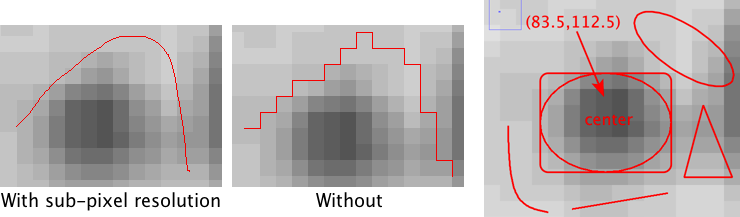
\includegraphics[scale=0.45]{images/SubPixel}\caption[Floating point selections]{\label{fig:Subpixel-selections}\textbf{Interpolated selections.}
ROIs drawn with (left) or without (middle) sub-pixel accuracy. For
line selections (\emph{see} \nameref{sec:Line-Selection-Tools}),
this option can be enabled in\textbf{ }\protect\userinterface{Edit\lyxarrow{}Options\lyxarrow{}\nameref{sub:Profile-Plot-Options...}}
by activating the \emph{Sub-pixel resolution} checkbox. Pixel coordinates
of area selections (\emph{see} \nameref{sec:Area-selection-tools}),
can be interpolated using \protect\userinterface{Edit\lyxarrow{}Selection\lyxarrow{}\nameref{sub:Interpolate}}.
The image on the right is the output of \protect\filenameref{\protect\href{http://imagej.nih.gov/ij/macros/js/SubPixelSelections.js}{SubPixelSelections.js}},
a script that demonstrates how to create selections at sub-pixel resolution
without the need of setting any option in ImageJ.}
\end{figure}



\calso{\nameref{sub:Zoom}, \nameref{sec:Magnifying-Glass}}


\section[Overlays]{Overlays\label{sub:Overlay-Intro}\improvement{Improved handling of Overlays}}

\index{Overlay}\index{Non-destructive annotations@Non-destructive annotations \see{Overlay,}}\index{Annotations!Non-destructive image overlay}Overlays
are non-active selections displayed `over' the pixel data, on the
image overlay, and are the core of non-destructive image processing
in ImageJ. In a way you can think of the image overlay as an invisible
\nameref{fig:The-ROI-Manager} in which selections are being added,
allowing ROIs to be on `hold'. This concept of multiple distinct
selections has been dramatically improved in \nameref{sub:ImageJ2intro}
so we urge you to download IJ2 if multiple ROIs are important in your
workflows.
\begin{figure}
\noindent 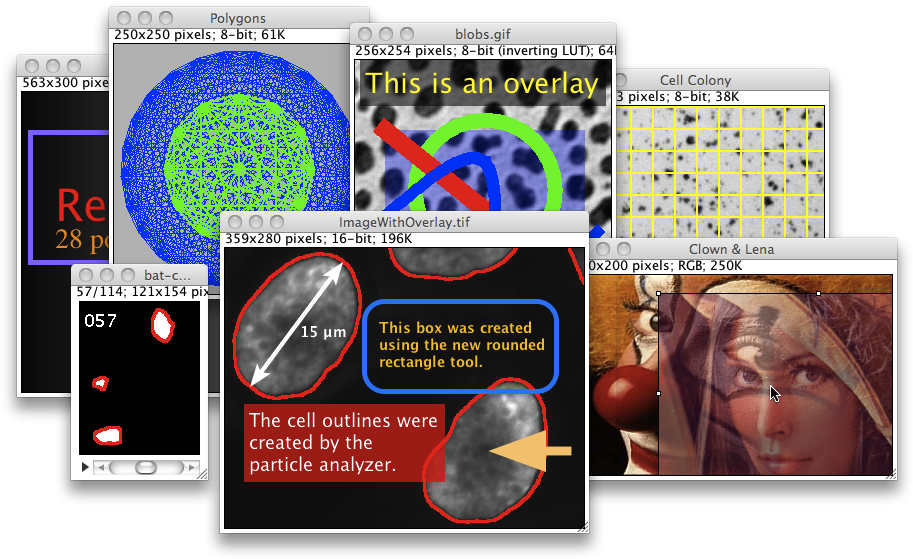
\includegraphics[width=0.75\columnwidth]{images/OverlayShowcase}\caption{\textbf{Non-destructive operations using the image overlay.} Overlays
can be used to annotate images, store ROIs and blend images (ImageROIs)
at multiple opacity levels. Refer to the \protect\userinterface{Image\lyxarrow{}\nameref{sub:Overlay}}documentation
for further \nameref{fig:image-overlays}. You can \protect\href{http://imagej.nih.gov/ij/docs/guide/images/ImageWithOverlay.tif}{download the frontmost}
image to practice overlay editing. }
\end{figure}


Importantly, overlay selections are \href{http://en.wikipedia.org/wiki/Vector_graphics}{vector graphics}
composed of mathematically-defined paths (as opposed to \href{http://en.wikipedia.org/wiki/Raster_graphics}{raster graphics}
in which objects are defined by pixels) and are not affected by scaling,
i.e., do not become pixelated. Most of overlay-related commands are
listed in the \userinterface{Image\lyxarrow{}\nameref{sub:Overlay}},
and in the ROI Manager window (\userinterface{Analyze\lyxarrow{}Tools\lyxarrow{}\nameref{sub:ROI-Manager...}}).
Appearance of overlay selections can be adjusted using \userinterface{Image\lyxarrow{}Overlay\lyxarrow{}\nameref{sub:Overlay-Options...}}/\userinterface{\nameref{sub:Labels...}}

As mentioned in \ref{infobox:Formats} \nameref{infobox:Formats},
overlays are saved in the header of tif images, and do not need to
be saved externally when using TIFF, the default file format of ImageJ.
The major advantages of overlays are summarized below:
\begin{description}
\item [{Storage\ of\ ROIs}] In ImageJ it is only possible to have a single
ROI at a time. However, it is possible to add selections to the image
overlay using \mykeystroke{B} (\userinterface{Image\lyxarrow{}Overlay\lyxarrow{}\nameref{sub:Add-Selection...[b]}}).\feature{}
Once added to the image overlay, ROIs can be re-activated by Alt-clicking,
Control-clicking or long-pressing ($\nicefrac{1}{4}$ second or longer).
Activated ROIs can be deleted by pressing the \mykeystroke{\noindent Backspace}
key. Selections can also be added and recovered in bulk, using the
\userinterface{Image\lyxarrow{}Overlay\lyxarrow{}\nameref{sub:From-ROI-Manager}}/\userinterface{\nameref{sub:To-ROI-Manager}}
commands.
\item [{Non-destructive\ annotations}] Overlays are the best way of annotating
images in ImageJ (\nameref{fig:image-overlays}). As vector graphics,
overlays do not change pixel values, can be scaled without loss of
quality even at high zoom levels (\emph{see} \ref{infobox:ZoomedCanvas}
\nameref{infobox:ZoomedCanvas}) and can be displayed at different
opacity values (\emph{see} \ref{infobox:HEX} \nameref{infobox:HEX}).
RGB snapshots of the image with embedded overlays can be created by
holding \mykeystroke{Shif} \mykeystroke{F}, the shortcut for \userinterface{Image\lyxarrow{}Overlay\lyxarrow{}\nameref{sub:Flatten-[F]}}.
`Flattened' images with the overlay rendered as pixel data are also
created when saving the image as PNG or JPEG (\userinterface{File\lyxarrow{}\nameref{sub:SaveAs}}),
or when printing the image canvas (\userinterface{File\lyxarrow{}\nameref{sub:Print...[p]}}).
The \userinterface{Flatten} command is also listed in the \nameref{fig:The-ROI-Manager}.
\item [{Image\ ROIs}] An \index{Image selection@Image selection \see{ImageROI}}\index{ImageROI}imageROI
(image selection) is a ROI that displays an image as an overlay. As
described in \userinterface{Edit\lyxarrow{}Selection\lyxarrow{}\nameref{sub:Image-to-Selection...}}
and \userinterface{Image\lyxarrow{}Overlay\lyxarrow{}\nameref{sub:Add-Image...}},
this allows multiple images to be \index{Blend}blended on a single
image canvas.
\end{description}

\section{3D Volumes\label{sub:3D-Intro}}

Currently, the support for \index{ThreeD ROIs@3D ROIs}\index{3D ROIs}3D
ROIs (selections containing contiguous cluster of voxels) is somewhat
limited in ImageJ. This limitation has been addressed by \nameref{sub:ImageJ2intro}
and several IJ1 plugins. The list below summarizes some of the ImageJ
plugins that deal effectively with multi-dimensional objects. Note
that a manual installation of these tools as standalone ImageJ plugins
is a challenging task given their special dependencies, reason why
they are all bundled as part of \index{Fiji}\nameref{sub:Fiji-intro}.
\begin{figure}
\noindent 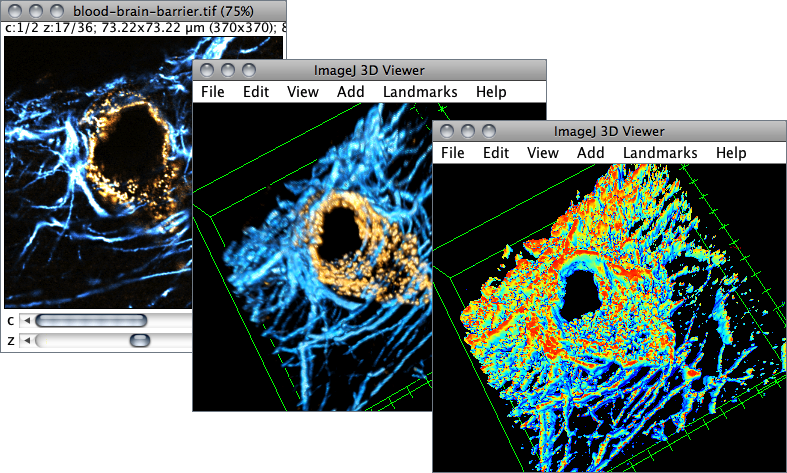
\includegraphics[width=0.7\columnwidth]{images/3Dviewer}\caption[3D Viewer]{\label{fig:-3D-Viewer}\textbf{3D Viewer (Fiji\,1.46o), bringing
hardware-accelerated 3D visualization to ImageJ.} As explained in
\nameref{sub:3D-Intro}, most of plugins that truly extend ImageJ
functionally to multi-dimentional data are bundled as part of Fiji.}
\end{figure}

\begin{description}
\item [{3D\ Filters}] Specialized \index{ThreeD Filters@3D Filters}\index{3D Filters}3D
filters such as \userinterface{Process\lyxarrow{}Filters\lyxarrow{}\nameref{sub:Gaussian-Blur-3D...}}
can be installed to perform 3D operations. Examples are the \href{http://imagejdocu.tudor.lu/doku.php?id=plugin:morphology:3d_binary_morphological_filters:start}{3D processing package}
by Thomas Boudier \cite{Iannuccelli:2010p13791} and the \href{http://fiji.sc/wiki/index.php/3D_Binary_Filters}{3D binary filters}
by Benjamin Schmid.
\item [{3D\ Object\ Counter}] \href{http://imagejdocu.tudor.lu/doku.php?id=plugin:analysis:3d_object_counter:start}{3D Object Counter}
(3D-OC) \index{ThreeD Object Counter@3D Object Counter}\index{3D Object Counter}counts
and qualifies 3D objects in a stack \cite{Bolte:2006p2466}, similarly
to the 2D analysis performed by \userinterface{Analyze\lyxarrow{}\nameref{sub:Analyze-Particles...}}
It is complemented by \href{http://imagejdocu.tudor.lu/doku.php?id=plugin:stacks:3d_roi_manager:start}{3D Roi Manager}
\cite{Iannuccelli:2010p13791}, a companion plugin that adds a 3D
\nameref{fig:The-ROI-Manager} to ImageJ
\item [{3D\ Viewer}] \href{http://3dviewer.neurofly.de/}{3D Viewer} \index{ThreeD Viewer@3D Viewer}\index{3D Viewer}brings
powerful hardware-accelerated 3D visualization to ImageJ \cite{Schmid:2010p18702},
extending the limited functionality of \userinterface{Image\lyxarrow{}Stacks\lyxarrow{}\nameref{sub:3D-Project...}}
In the ImageJ \nameref{fig:-3D-Viewer} stacks can be displayed as
texture-based volume renderings, surfaces or orthoslices. It is macro-recordable
and can be used by other plugins as a high-level programming library
for 3D visualization
\item [{Simple\ Neurite\ Tracer}] \href{http://fiji.sc/wiki/index.php/Simple_Neurite_Tracer}{Simple Neurite Tracer}
\index{Simple Neurite Tracer}allows semi-automated segmentation of
tubular structures in 3D \cite{Longair:2011p20768}
\item [{TrakEM2}] As mentioned earlier, \nameref{misc:TrakEM2} \index{TrakEM2}features
powerful tools for multi-dimensional regions of interest \cite{Cardona:2010p18306}
\end{description}

\calso{\userinterface{Image\lyxarrow{}Stacks\lyxarrow{}\nameref{sub:3D-Project...}}/\userinterface{\nameref{sub:Orthogonal-Views}},
\userinterface{Analyze\lyxarrow{}\nameref{sub:Surface-Plot...}},
\ref{infobox:Skeletonize-vs-Skeletonize3D} \nameref{infobox:Skeletonize-vs-Skeletonize3D},
\href{http://fiji.sc/wiki/index.php/Special:Search?search=3d&fulltext=Search}{3D tools in Fiji},
\href{http://www.longair.net/edinburgh/imagej/three-pane-crop/}{Three Pane Crop},
\href{http://imagejdocu.tudor.lu/doku.php?id=tutorial:working:3d_image_processing_and_analysis_with_imagej}{3D image processing tutorials}
on the ImageJ wikipage}


\section[Settings and Preferences]{Settings and Preferences\label{sec:Settings-and-Preferences}\improvement{}}

\index{Settings}\index{Preferences@Preferences \see{Settings,}}\index{Options@Options \see{Settings,}}ImageJ
preferences are automatically saved in a preferences file, the\texttt{
}\filenameref{IJ\_prefs.txt} text file. This file is stored in \dirnameref{$\sim$/Library/Preferences/}
on Mac OS\,X, in \dirnameref{$\sim$/.imagej/} on Linux and in the
ImageJ folder on Windows. Several macros and plugins also write parameters
to this file. If the \filenameref{IJ\_prefs.txt} is erased using
\userinterface{Edit\lyxarrow{}Options\lyxarrow{}\nameref{sub:ResetOptions}},
ImageJ will create a new one the next time it is opened resetting
all parameters to their default values. 

Sometimes, it may be useful to override (or restore) certain settings
that may have been changed during a working session. For example,
the \emph{Limit to threshold} option (\userinterface{\textsf{Analyze\lyxarrow{}}\nameref{sub:Set-Measurements...}})
will affect most measurements performed on thresholded images. Thus,
it may be wise to check the status of this parameter before each analysis,
specially when working on multiple computers.

\begin{lstlisting}[caption={Ensuring Specific Settings at Launch},label={lis:setOption},float=h,showstringspaces=false,tabsize=4]
 macro "AutoRun" {
   setOption("DebugMode", true);
   setOption("Bicubic", true);
   setOption("Display Label", true);
   setOption("Limit to Threshold", false);
   setOption("BlackBackground", true);
   run("Colors...", "foreground=white background=black"); //this line could be substituted by: setBackgroundColor(0,0,0); setForegroundColor(255,255,255);
   run("Profile Plot Options...", "width=350 height=200 draw");
   run("Brightness/Contrast...");
 }
\end{lstlisting}
The \texttt{\code{\texttt{setOption()}}} \href{http://imagej.nih.gov/ij/developer/macro/functions.html\#setOption}{macro function}
can be used to set this and several other ImageJ options. Calling
this function from the \index{StartupMacros}\index{AutoRun}``AutoRun''
macro in the \filenameref{StartupMacros.txt} file ensures preferences
are set each time ImageJ starts. The macro \eqref{lis:setOption}
\nameref{lis:setOption} exemplifies this approach ensuring that the
following settings are enforced at startup:
\begin{enumerate}
\item TIFF tag values are displayed by ImageJ (\emph{Debug Mode} in \textsf{\userinterface{\textsf{Edit\lyxarrow{}Options\lyxarrow{}}\nameref{sub:Misc...}}})
\item Bicubic interpolation is preferred over bilinear (e.g.,\textsf{ }\userinterface{\textsf{Edit\lyxarrow{}Selection\lyxarrow{}}\nameref{sub:Straighten...}})
\item The name of the measured image name is recorded in the first column
of the \nameref{sec:Results-Table} (\emph{Display Label }in \userinterface{\textsf{Analyze\lyxarrow{}}\nameref{sub:Set-Measurements...}})
\item Measurements are not restricted to thresholded pixels (\emph{Limit
to Threshold} in \userinterface{\textsf{Analyze\lyxarrow{}}\nameref{sub:Set-Measurements...}})
\item Binary images are processed assuming white objects on a black background
(\emph{Black background} in \userinterface{\textsf{Process\lyxarrow{}Binary\lyxarrow{}}\nameref{sub:BinaryOptions...}},
\emph{see} \ref{infobox:blackBackground} \nameref{infobox:blackBackground})
\item \emph{Background color} is black and \emph{foreground color} is white
(\textsf{\userinterface{\textsf{Edit\lyxarrow{}Options\lyxarrow{}}\nameref{sub:Colors...}}})
\item ImageJ plots contain grid lines and are always $350\times200$\,pixels
in size (\textsf{\userinterface{\textsf{Edit\lyxarrow{}Options\lyxarrow{}}\nameref{sub:Profile-Plot-Options...}}})
\item Open the B\&C widget at its last saved screen position (\textsf{\userinterface{\textsf{Image\lyxarrow{}Adjust\lyxarrow{}}\nameref{sub:Brightness/Contrast...[C]}}})
\end{enumerate}

\calso{\nameref{sec:GUIcustomization}, FAQs\nomenclature{FAQ}{Frequently Asked Questions}
on \href{http://imagejdocu.tudor.lu/doku.php?id=faq:technical:how_do_i_set_up_imagej_to_deal_with_white_particles_on_a_black_background_by_default}{ImageJ wikipage},
\ref{infobox:Organizing-Commands} \nameref{infobox:Organizing-Commands} }
